5G forwarding plane and the relevant network functions are 
briefly reviewed in \ref{sec:5GfwdPlane}. PFCP protocol and its 
significance is discussed in \ref{sec:PFCP}. 
The layout of the report is outlined in \ref{sec:Organization}. 

\section {5G Forwarding Plane \label{sec:5GfwdPlane}}
The major difference in  data packet processing between 5G and earlier standards is control-user plane 
separation and the use of network function virtualization. Forwarding of packets (user plane), 
authentication of mobile devices (control plane), session establishment and management (control plane) are some of the network 
functions required in the core of a telecommunication network. These network functions run on different or same physical machines as 
virtual machines (preferably) for easier migration/scaling.

This project is mainly concerned with data forwarding plane. The network functions in our implementation will 
run as separate processes. The network functions relevant for forwarding plane are described further.
\subsection{Radio Access Network (RAN) \label{sec:RAN}} 
RAN is a point of contact for all the user equipments (UEs) like handsets, IOT devices, industrial machine controllers etc. 
RAN runs on all the mobile towers and UEs communicate with the one in their vicinity. RAN is
 responsible for talking to Access Mobility Function for authenticating the UEs, registering the  new
  session. The session establishment request is further forwarded to Session Management Function
  (SMF) which establishes a new session and forward session information to the User Plane Function (UPF). 
  \subsection{User Plane Function (UPF) \label{sec:UPF}}
  User plane function (UPF) is responsible for forwarding packets from user equipments to the
   Internet and vice versa. The uplink direction is defined as the flow of the packets from user
    equipments to the Internet. The downlink direction is defined as the traffic coming from the Internet  to the user equipments/RAN. 
  
 \begin{figure}[htbp]
    \centering
    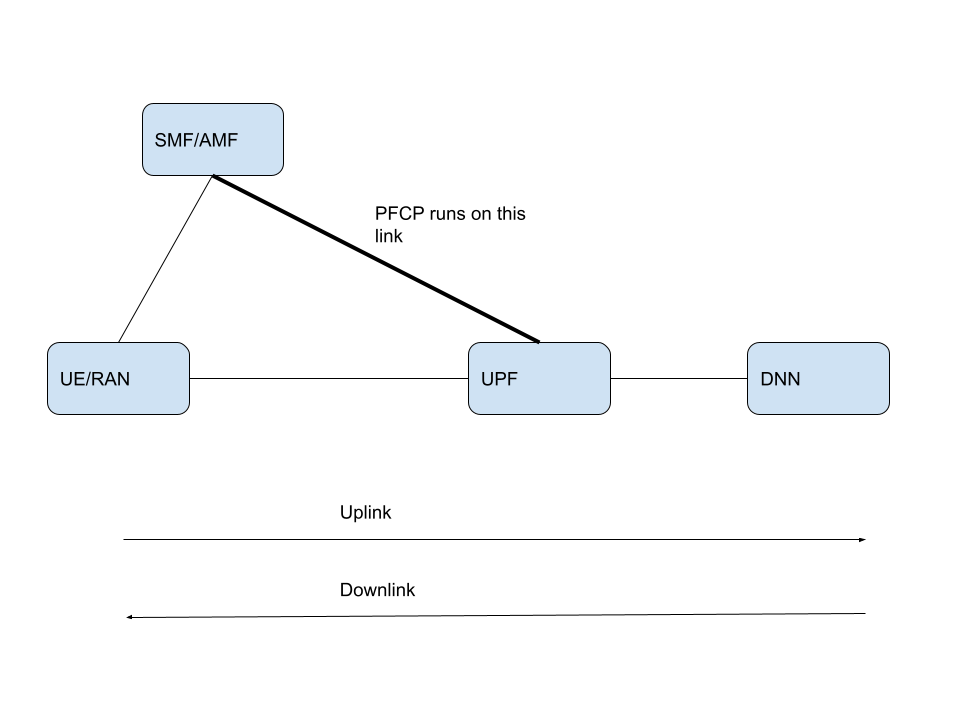
\includegraphics[width=0.7\textwidth, keepaspectratio]{./fig/Introduction/5GSecond.png}
    \caption{5G Forwarding Plane}
    \label{fig5Gforwarding}
\end{figure}
\subsection{Data Network Name (DNN) \label{sec:DNN}}
This network function is the gateway to the public Internet. All incoming packets from outside the
 local network are received by this NF and are subsequently forwarded to the user equipment through
   the UPF and the RAN. 

\section {PFCP Protocol\label{sec:PFCP}}
 \begin{figure}[htbp]
    \centering
    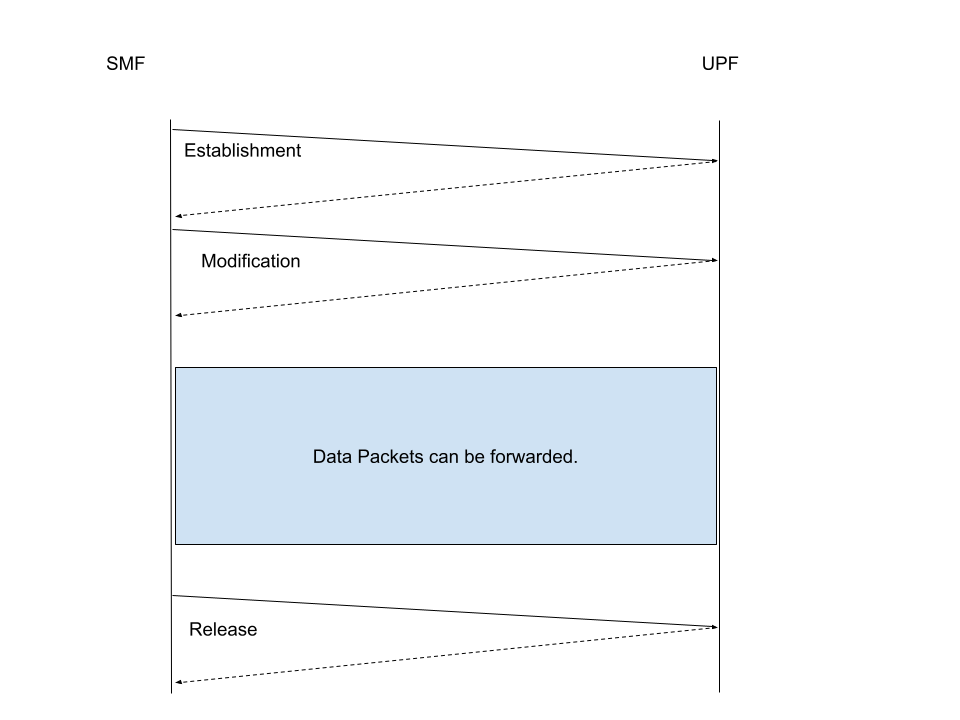
\includegraphics[width=0.7\textwidth, keepaspectratio]{./fig/Introduction/PFCP.png}
    \caption{PFCP Session Messages}
    \label{fig:PFCP}
\end{figure}

PFCP stands for Packet Forwarding Control Protocol. 
 There are two types of messages sent using PFCP - node related and session related.
 The discussion here describes session related messages.

 Session Management Function (SMF) interacts with the User Plane Function (UPF) to setup sessions related 
 information at the UPF.
This  information enables UPF to identify data packets of different sessions coming from RAN 
and provide forwarding, usage report, charging, buffering, QoS related service to the sessions.
Each session is identified by a unique session ID which helps in differentiating 
among different UEs/sessions at the UPF. 

There are three kinds of messages sent from SMF to the UPF in PFCP session related messages-
\begin{itemize}
	\item \textbf{Establishment Request} This message has all the forwarding, usage report, QoS etc. related information for  a new UE session.  
	\item \textbf{Modification Request} Once the establishment response is
	received from the UPF, the UPF sends the modification request. The important field in this message is the intimation of identifier that will be used for data plane packets coming from the UPF. The data forwarding can not start before the modification response is received.
	\item \textbf{Release Request} Once the session is not required, th release 
	request is sent to the UPF signaling the tear down of the session and UPF
	 may remove this session's related information.
\end{itemize}
UPF gives response to each of the three messages. 

\section {Organization \label{sec:Organization}}

The report is organized as follows.
The chapter \ref{chap:ProblemStatement} defines the problem statement. Chapter 
\ref{chap:RANDesign} discusses the  design of the RAN emulator describing the core
 layout, how control plane messages are forwarded and what are the different modes
  of operation. Control plane latency calculation mechanisms are explained in  the
   Chapter \ref{chap:CPLatency}. Chapter \ref{chap:CPDPTraffic} describes the
    simultaneous forwarding of control plane and data plane traffic. Chapter 
    \ref{chap:CleanCode}  describes the steps taken to clean the code and make it easy to extend for future developers. 
    The results generated from control plane latency experiments with different models of the UPF and simultaneous transfer of control plane and data plane traffic are reported in Chapter \ref{chap:Results}.